\documentclass[
  lualatex,
  aspectratio=169,
  14pt
]{beamer}

\usetheme[progressbar=frametitle]{Metropolis}
\setbeameroption{show notes on second screen=bottom}

\usepackage{xparse}
\usepackage{mathtools,amssymb}
\usepackage{graphicx,xcolor}
\usepackage{pxrubrica}
\usepackage{calc}
\usepackage[absolute,overlay]{textpos}
\usepackage{enumitem}
\usepackage[1.7]{bxpdfver}
\usepackage{pdfcomment}

% フォント
\usepackage[lining,tabular,sfdefault]{FiraSans}
\usepackage[mathrm=sym,mathbf=sym]{unicode-math}
\setmathfont{Fira Math}
\usepackage[no-math,deluxe,haranoaji]{luatexja-preset}
\RenewDocumentCommand\kanjifamilydefault{}{\gtdefault}

\usepackage{hyperref}

\title{世も令和になって久しいので\\オレオレIP電話網や黒電話で遊んでみる}
\subject{CS集会\#47}
\author{上羽 未栞(a.k.a. KusaReMKN)}
\institute{%
  \url{https://KusaReMKN.com/}\\
  Twitter: \href{https://twitter.com/KusaReMKN}{@KusaReMKN}}
\keywords{黒電話; VoIP; IP電話; MikoPBX; 東京広域電話網}
\date{2025-03-11}

\begin{document}

\begin{frame}
  \titlepage
  \note{
    発表を始めるよ。

    「世も令和になって久しいのでオレオレIP電話網や黒電話で遊んでみる」と題して、
    みかんちゃんが発表するよ。
  }
\end{frame}

\begin{frame}
  \frametitle{今回のおはなし}

  ~\\[-.25\baselineskip]
  \tableofcontents
  \note{
    今回の発表の流れはこんな感じだよ。
    質疑応答を含めて大体20分間くらいで進められたらいいな。
  }
\end{frame}

%\begin{frame}
%  \frametitle{今日のレジュメ(宣伝(1回目))}
%
%  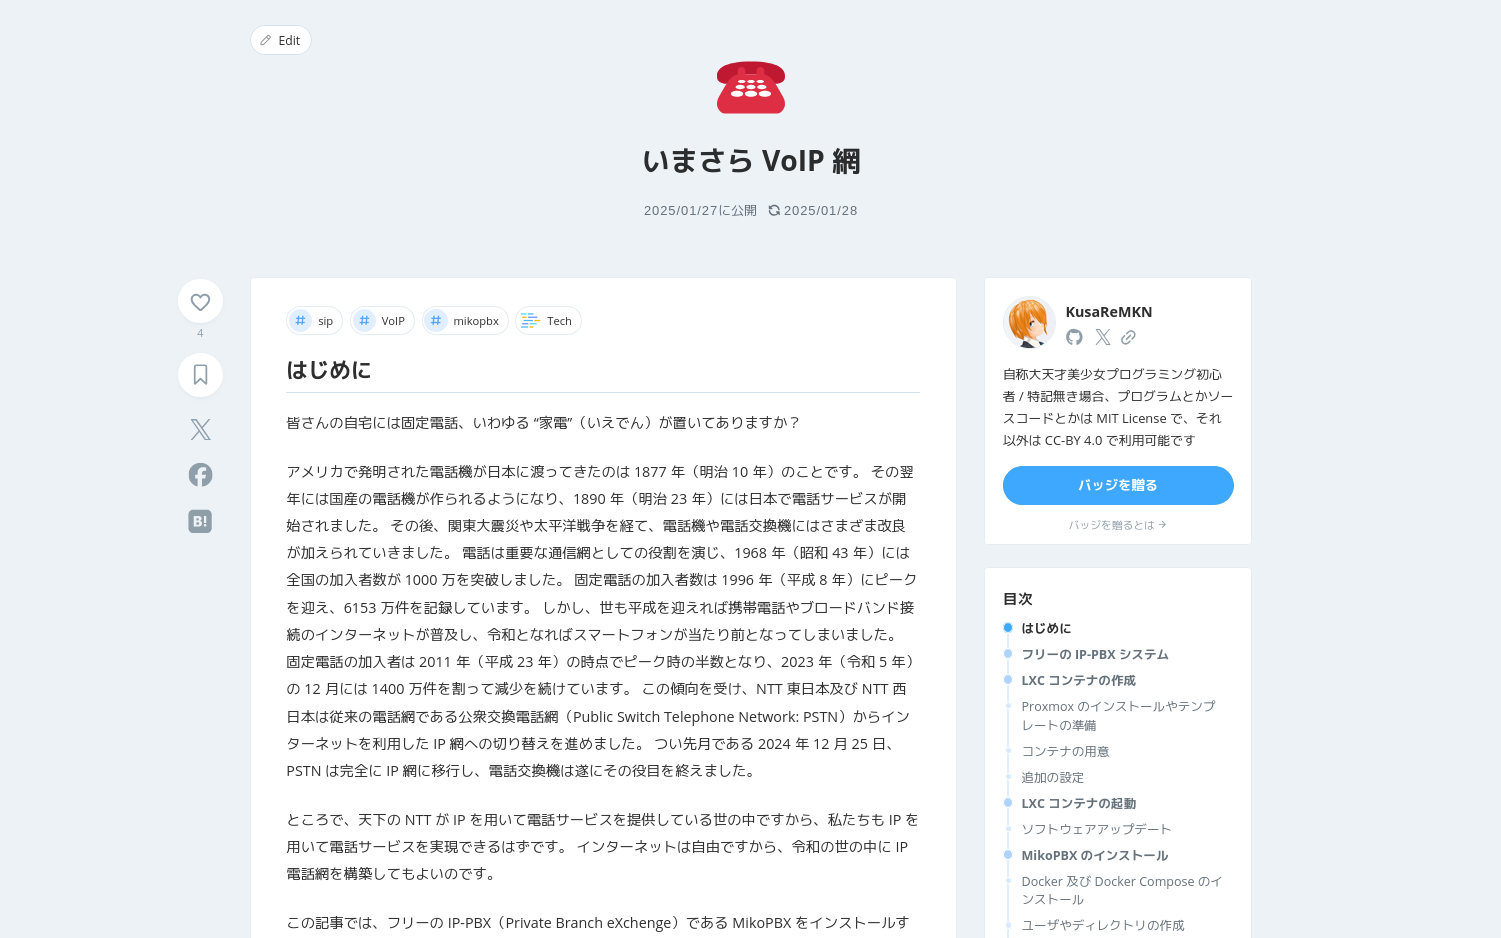
\includegraphics[width=\linewidth]{./images/imasara.png}
%  \note{
%    早速だけど、宣伝だよ(えっ)。
%    今回の発表内容についての記事がZennに投稿されているよ。
%  }
%\end{frame}
%
%\begin{frame}
%  \frametitle{今日のレジュメ(宣伝(1回目))}
%
%  \begin{description}[labelwidth=\linewidth,itemsep=\zh]
%    \item[いまさらVoIP網]
%      {\small
%      \url{https://zenn.dev/kusaremkn/articles/abd760f9f2f450}}
%    \item[VoIPルータを使って黒電話をIP電話機にする]
%      {\small
%      \url{https://zenn.dev/kusaremkn/articles/187222dc1d4f1d}}
%    \item[ICOM VE-TA10を使うためにパケットを書き換えたりする]
%      {\small
%      \url{https://zenn.dev/kusaremkn/articles/cb32b500fc1334}}
%  \end{description}
%  \note{
%    関連するトピックについての記事も投稿されているよ。
%    暇な人は読んでみてね。
%    「いまさらVoIP網」でGoogleすると一番上の方に出てくるよ。
%  }
%\end{frame}

\section*{みかんちゃんについて}
\note{
  自己紹介するよ。
}

\begin{frame}
  \frametitle{自称・大天才美少女プログラミング初心者}

  \begin{textblock*}{0.5\paperwidth}(0.6cm, 3.5cm)
    
\includegraphics[width=0.3\paperwidth]{./images/mikanchan.png}
  \end{textblock*}
  \begin{columns}
    \begin{column}{0.30\textwidth}
      \\~\\[-.25\baselineskip]
    \end{column}
    \begin{column}{0.69\textwidth}
      \\~\\[-.25\baselineskip]
      「\ruby{上羽}{うわ|ば} \ruby{未栞}{み|かん}」
      あるいは「\ruby[g]{KusaReMKN}{くされみかん}」\\
      \hspace{1.5\zw}\textbf{みかんちゃん}って呼んでね!
      \\~\\[-.5\baselineskip]

      \newlength{\zeropeke}
      \settowidth{\zeropeke}{\tiny 0x}
      \hspace{-\zeropeke}{\tiny 0x}18\nobreak 歳のJK(重要)
      \\~\\[-.5\baselineskip]

      実はプログラマでもエンジニアでもない\\
      \hspace{1.5\zw}古い計算機っぽいものが大好き
      \\~\\[-.5\baselineskip]

      Twitterで思想を垂れ流すことが得意\\
      \hspace{1.5\zw}\url{https://kusaremkn.com/}も見てね
    \end{column}
  \end{columns}
  \note{
    大天才美少女プログラミング初心者を自称している、上羽未栞だよ。
    みかんちゃんって呼ばれると大変喜ぶよ。
    イチハチ歳のJKだよ。

    大天才とかプログラミング初心者とか言っているけれど、
    実はプログラマでもエンジニアでもないよ。
    外の人(学生のすがた)は通信方式について研究していたりするけれど、
    それはまた別のお話だよ。
    それはそれとして古い計算機っぽいものが大好きだよ。
    よくハードオフに出没してジャンク箱を小豆洗いしているよ。

    Twitterとかウェブサイトとかあるよ。
    暇な人は覗いてみてね。
    深淵があるよ。
  }
\end{frame}

\section{「でんわ」のはじまり}
\note{
  早速「でんわ」についてお話していくよ。
}

\begin{frame}
  \frametitle{HARD OFFに売られていた黒電話(白色)}

  \centering
  \includegraphics[height=.85\textheight]{./images/ivory.jpeg}
  \note{
    いつものようにハードオフをふらついていると黒電話(白色)が現れたよ。
    最初はにらめっこをしているだけだったんだけど、
    気付いたら財布の中身が軽くなって手元に電話機が発生していたよ。
    これがみかんちゃんと「でんわ」との邂逅だよ。
  }
\end{frame}

\begin{frame}
  \frametitle{一方そのころ、限界セルフホスティング界隈では……}

  \begin{columns}[c]
    \begin{column}[c]{.80\textwidth}
      \ruby[g]{\bfseries MMTNET}{ももたねつと}:\\
      \hspace{1.5\zw}Malleable Mutual Tunneling Network\\
      \hspace{1.5\zw}for Experimental Technologies
      \\~\\[-.5\baselineskip]

      SoftEther VPNを使ってホストを相互接続\\
      \hspace{1.5\zw}自作インターネットを目論んでいた
      \\~\\[-.5\baselineskip]

      MMTNET上で動作するアプリケーション\\
      \hspace{1.5\zw}黒電話を利用したIP電話が挙げられていた\\
      \hspace{1.5\zw}MMTNETの前身(HVCAN)でも運用されていた
    \end{column}
    \begin{column}{.17\textwidth}
      \centering
      \\~\\[-.75\baselineskip]
      
\includegraphics[width=\linewidth]{./images/pepepper.jpg}

      
\includegraphics[width=\linewidth]{./images/yude.jpg}

      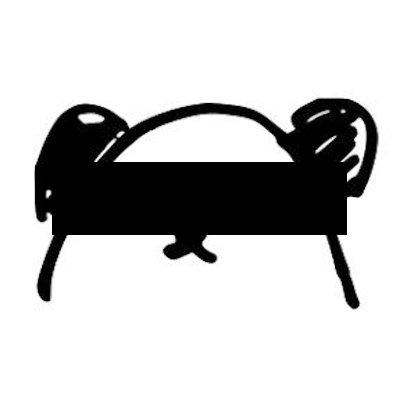
\includegraphics[width=\linewidth]{./images/kurari.jpg}
    \end{column}
  \end{columns}
  \note{
    みかんちゃんが「でんわ」と邂逅している一方、
    限界セルフホスティング界隈(スライド右側の人々)では
    MMTNETとかいうけしからんネットワークが構築されようとしていたよ。
    MMTNETはSoftEther VPNを利用したネットワークで、
    この上で自作のインターネットを作ることを目論んでいたよ。

    このMMTNET上で動作するアプリケーションとして、
    黒電話を利用したIP電話が挙げられていたよ。
    これはどういうことかというと、
    MMTNETの前身にあたるネットワークとして
    HVCANという異常ネットワークがあるんだけど、
    これの上で黒電話IP電話が実現していたので、
    これをもっと発展させてみよいうという話だったよ。
  }
\end{frame}

\begin{frame}
  \frametitle{HVCAN上のIP電話発足の貴重なシーン}

  ~\\[-.75\baselineskip]
  \begin{columns}[b]
    \begin{column}{.49\textwidth}
      \centering
      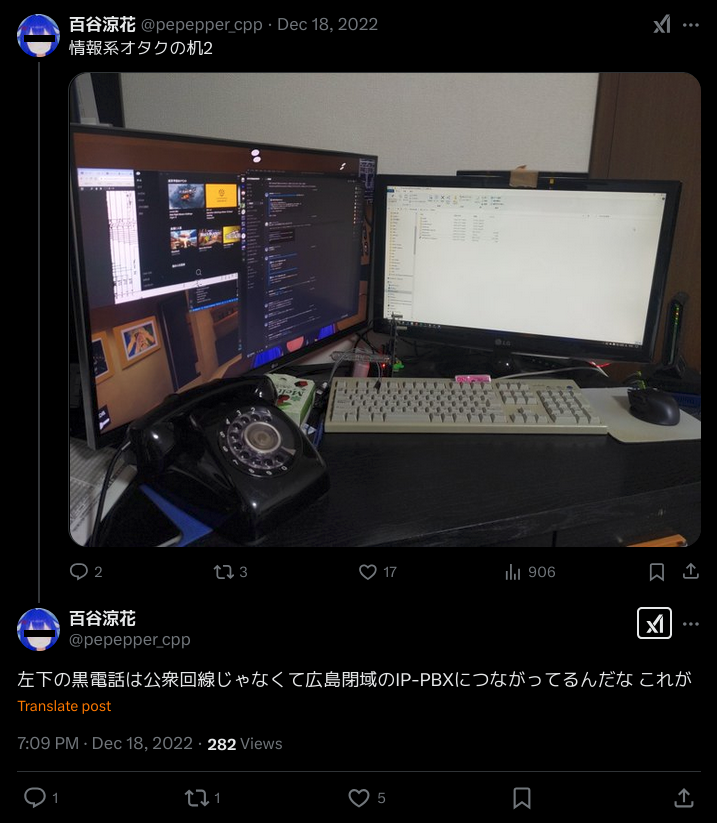
\includegraphics[height=.9\textheight]{./images/ijyou.png}
    \end{column}
    \begin{column}{.49\textwidth}
      \centering
      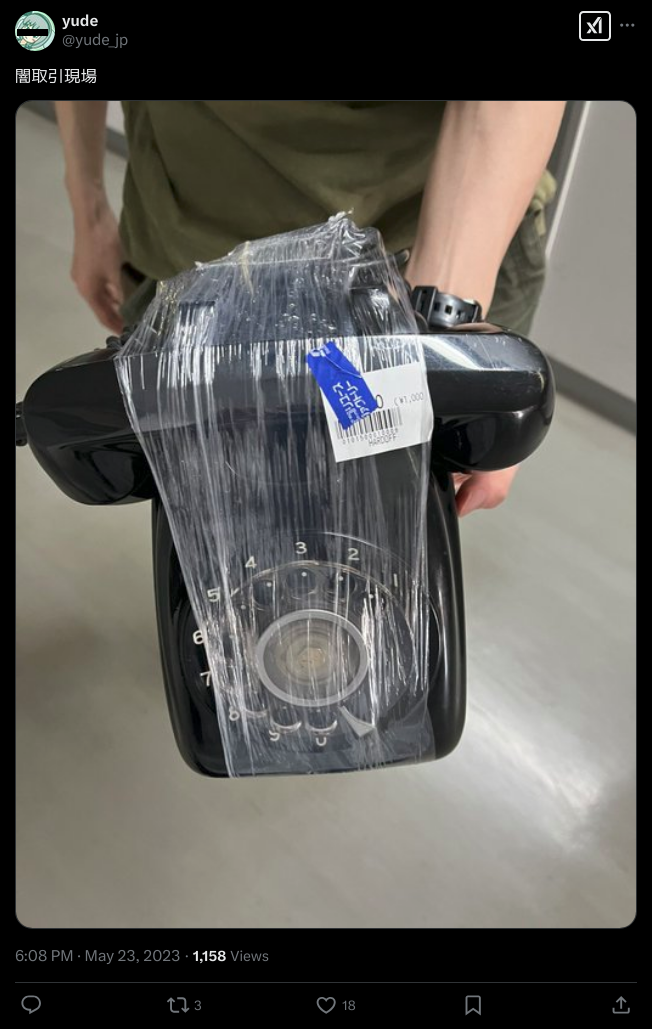
\includegraphics[height=.9\textheight]{./images/yami.png}
    \end{column}
  \end{columns}
  \note{
    HVCANでIP電話が実現されていたことを確認するためにツイートを遡ってみたよ。
    うん、確かに異常オタクの机に黒電話は存在しているし、
    しかもハドフで得た黒電話を取引している怪しい現場写真まで出てきたよ。
  }
\end{frame}


\begin{frame}
  \frametitle{HVCAN上の電話網(?)の様子}

  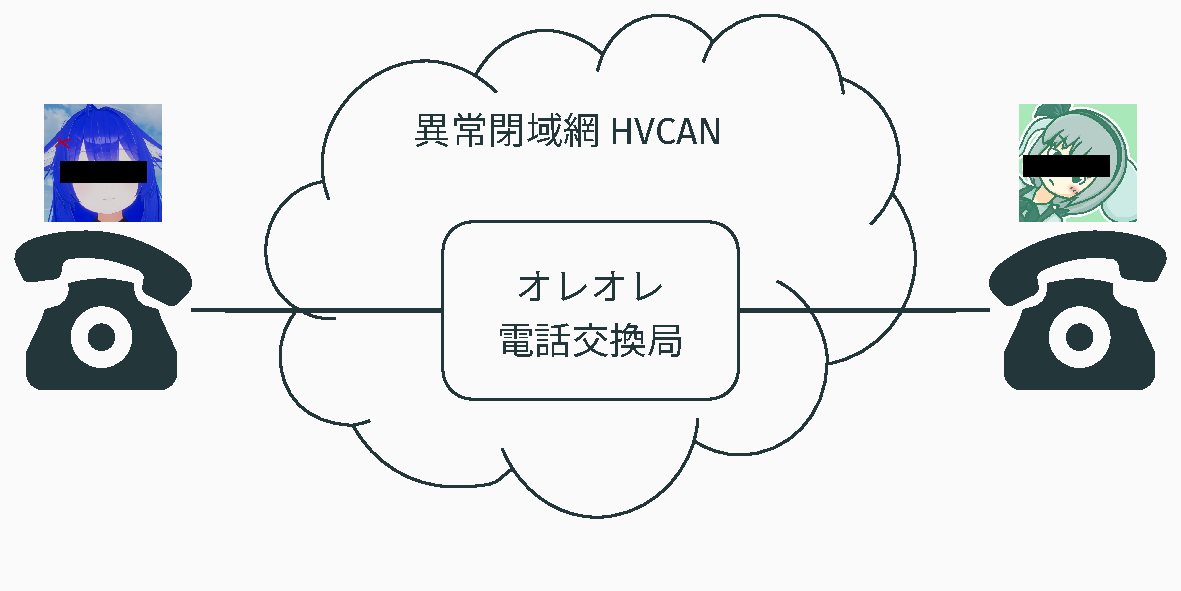
\includegraphics[page=1,width=\linewidth]{./images/pictures.pdf}
  \note{
    HVCANの上で実現していたIP電話のシステムを図に起こすとこんな感じになるよ。
    HVCANには単一の交換局があって、
    これに全ての端末(電話機)が接続されていたよ。
    つまり、事実上の内線電話に留まっていたよ。
  }
\end{frame}

\begin{frame}
  \frametitle{実現したいこと}

  \begin{description}[labelwidth=\linewidth,itemsep=.25\zh]
    \item[外線通話と多局接続]
      交換局をまたぐ通話\\
      複数の交換局の相互接続
    \item[交換局ホップ]
      相互接続されていない局の通話
  \end{description}

  状況を簡単にするためMMTNETから切り離される\\
  \hspace{1.5\zw}オレオレ電話網「\textbf{東京広域電話網}」の爆誕
  \note{
    というわけで、今回実現したいことは次の二つだよ。
    一つ目は外線通話、多局接続の実現だよ。
    これは交換局をまたぐような通話であったり、
    沢山の交換局が相互に接続された電話網を構築したりする部分にあたるよ。
    二つ目は交換局ホップだよ。
    後のスライドでも述べるけれども、
    交換局が増えてくると全ての局を直接相互接続することが現実的ではなくなってくるよ。
    これを解決するために、直接接続されていない局同士でも通話できるようにするよ。

    これがMMTNET上にあると、多くの人類のためにならないよ。
    多くの人間はMMTNET上にいないからだよ。
    そのため、MMTNETから電話網の部分を切り出して電話網単体の問題として解決することにしたよ。
    オレオレ電話網「東京広域電話網」が爆誕したよ。
  }
\end{frame}

\section{外線通話と多局接続}
\note{
  一つ目の問題である外線通話と多局接続について考えるよ。
}

\begin{frame}
  \frametitle{基本の構成}

  \begin{columns}
    \begin{column}{.6\textwidth}
      交換局として\textbf{MikoPBX}を用いる\\
      \hspace{1.5\zw}AsteriskベースのIP-PBXシステム\\
      \hspace{1.5\zw}シンプルなWEB UIが魅力
      \\~\\[-.5\baselineskip]

      スタンドアロン版とDocker版がある
    \end{column}
    \begin{column}{.39\textwidth}
      
\includegraphics[width=\linewidth]{./images/mikopbx.png}
    \end{column}
  \end{columns}
  \note{
    まずは交換局の構成について説明するよ。
    今回の電話網構築にはフリーのPBXシステムであるMikoPBXを用いるよ。
    これはAsteriskというIP-PBX(要はIP電話の交換局システム)をベースとしたシステムだよ。
    シンプルなWEB UIが魅力だよ
    (つまり他のPBXシステムにはシンプルでないWEB UIをもつものがあるということだよ)。
    MikoPBXにはスタンドアロン版とDocker版があるので使い分けられるよ。
  }
\end{frame}

\begin{frame}
  \frametitle{ダメなシステム構成(その1)}

  \includegraphics[page=2,width=\linewidth]{./images/pictures.pdf}
  \note{
    まずはスタンドアロン版を使うことを考えてみるよ。
    これが最も簡単な構成であるのだけれど、
    これはちょっとむつかしくて、
    交換局はグローバルなインターネットに晒されなければならないよ。
    セキュリティ的にも嫌な気持ちになるし、
    そもそも全ての局がグローバルなIPアドレスを持たなければならなくて、
    現実的じゃないね。
  }
\end{frame}

\begin{frame}
  \frametitle{VPNを使えばいいじゃない}

  \begin{columns}
    \begin{column}{.6\textwidth}
      交換局間の接続に\textbf{Tailscale}を用いる\\
      \hspace{1.5\zw}簡単なメッシュ型VPNサービス\\
      \hspace{1.5\zw}ユーザ間で接続を共有できてお得
    \end{column}
    \begin{column}{.39\textwidth}
      
\includegraphics[width=\linewidth]{./images/tailscale.png}
    \end{column}
  \end{columns}
  \note{
    インターネットに晒すことが問題であるならば、
    VPNを使えばこの問題を解決できそうだよ。
    今回はTailscaleを使うことを考えたよ。
    Tailscaleは大変すばらしいメッシュ型のVPNサービスだよ。
    みんなも使ったことあるかも(?)
    ユーザ内のVPNを作ることもできるし、
    VPN上のホストを他のユーザと共有できたりしてお得だよ。
  }
\end{frame}

\begin{frame}
  \frametitle{ダメなシステム構成(その2)}

  \includegraphics[page=3,width=\linewidth]{./images/pictures.pdf}
  \note{
    なるほど、Tailscaleを使えば完璧だ、と思ったけどやっぱりこれもダメだったよ。
    スタンドアロン版のMikoPBXはLinuxディストリみたいに
    完結したシステムとして提供されるのだけれど、
    この上でTailscaleのクライアントソフトを動かせそうにないことがわかったよ。
    クライアントソフトが動かないとTailscale越しの接続を実現できるハズもないので、
    これではいけないね。
  }
\end{frame}

\begin{frame}
  \frametitle{Docker版を使えばいいじゃない}

  \begin{columns}
    \begin{column}{.6\textwidth}
      \textbf{Docker}版MikoPBXを用いる\\
      \hspace{1.5\zw}ホスト側でTailnetに接続\\
      \hspace{1.5\zw}MikoPBX側は何も考えなくてよい
    \end{column}
    \begin{column}{.39\textwidth}
      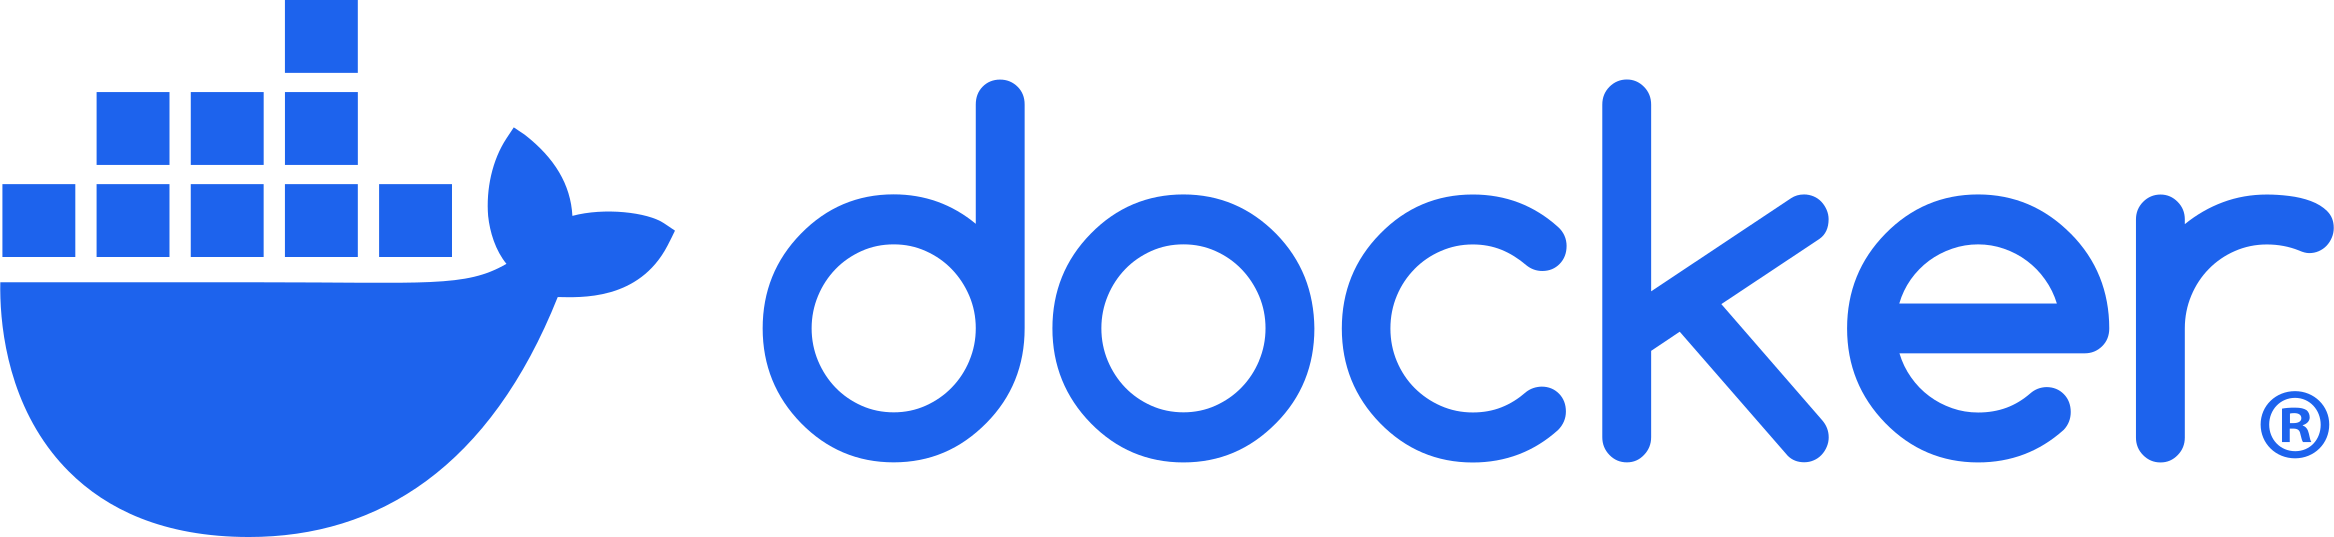
\includegraphics[width=\linewidth]{./images/docker.png}
    \end{column}
  \end{columns}
  \note{
    ところで、ちょっと思い出してみるとMikoPBXにはDocker版があったね。
    これを使うと簡単に構成できそうだよ。
    Dockerコンテナを動かすホスト環境(これは普通Ubuntuだよ)で
    Tailscaleのクライアントソフトを動かすことは容易いよ。
    この環境の上に構築されるMikoPBXは
    当然Tailscaleのネットワークに接続できるので、
    特段むつかしいことを考える必要がないよ。
  }
\end{frame}

\begin{frame}
  \frametitle{完成版のシステム構成}

  MikoPBXの設定をこねくり回していたら外線通話が可能に!

  \includegraphics[page=4,width=\linewidth]{./images/pictures.pdf}

  \note{
    というわけで完成版のシステム構成がこんな感じだよ。
    Ubuntuとかの上にTailscaleをインストールして
    Tailnet経由で接続できるようにしておくよ。
    この上にDocker環境を用意して、
    その上にDocker版のMikoPBXをインストールするよ。

    この構成にして、
    MikoPBXの設定をこねくり回すこと二三日していたら外線接続が実現できたよ。
    (東京と横浜との交換局が繋がったときみたいな感動があるね(は?))

    (2024-11-11)
  }
\end{frame}

\begin{frame}
  \frametitle{内線接続・外線接続が完了(追加スライド)}

  \vspace{\baselineskip}
  \includegraphics[page=8,width=\linewidth]{./images/pictures.pdf}

  \note{
    これまでできていた同一局内の端末同士の内線通話に加えて、
    局をまたいで別の局の端末との通話(外線通話)もできるようになったよ。
  }
\end{frame}

\begin{frame}
  \frametitle{多局接続がむつかしい}

  \includegraphics[page=5,width=\linewidth]{./images/pictures.pdf}
  \note{
    さて、外線通話の実現はできたわけだけれども、
    多数の交換局が相互に接続できるようになるには少しだけ時間が掛かったよ。
    というのも、局Aと局Bとがあってこれらが接続済のときに、
    局Cが局Aに接続しようとするとなぜか拒否されてしまうという問題が発生していたよ。
  }
\end{frame}

\begin{frame}
  \frametitle{WEBに表示されていない設定項目}

  \begin{columns}
    \begin{column}{.7\textwidth}
      MikoPBXのWEB UIで設定を変更すると\\
      \hspace{1.5\zw}システムの設定ファイルが書き変わる
      \\~\\[-.5\baselineskip]

      WEB UIに表示されていない項目もある\\
      \hspace{1.5\zw}設定項目\texttt{max\_contacts}\\
      \hspace{1.5\zw}デフォルトの値は\textbf{1}\\
      \hspace{1.5\zw}これを100にすると接続できる
    \end{column}
    \begin{column}{.29\textwidth}
      
\includegraphics[width=\linewidth]{./images/jiminy.jpg}
    \end{column}
  \end{columns}
  \note{
    この問題を解決する鍵はもっと下側の層にあったよ。
    MikoPBXのWEB UIで設定を変更すると、
    その下側で動作しているAsteriskシステムの設定ファイルが書き変わるよ。

    異常オタクがこれについてめちゃくちゃ調査をしたところ原因がわかったよ。
    設定項目のうち、システムの動作に関わるいくつかの項目はWEB UI上に表示されていなかったよ。
    この設定項目がmax\_contactsだよ。
    この項目のデフォルトの値は1で、つまり同時に接続を受ける局の数は1に制限されていたよ。
    設定ファイルを直接書き換えてこの値を100とか1000とかに変更すると接続できるようになったよ。
    これで電話「網」を構築できるようになったよ。(2024-11-23)
  }
\end{frame}

\section{交換局ホップ}
\note{
  次に二つ目の問題である交換局ホップについて考えるよ。
}

\begin{frame}
  \frametitle{新しい局を追加する際の手間}

  \includegraphics[page=6,width=\linewidth]{./images/pictures.pdf}
  \note{
    電話網を構築できることがわかると、電話網は急速に発展していったよ。
    ここで問題になってきたのが新しい電話局を追加するときの手間だよ。
    電話局は相互に接続されていないと通話ができなかったので、
    例えば局Fが新しく網A--Eに接続しようとすると、
    全ての局で設定を行う必要があったよ。
    これはもう大変面倒だし、
    今後の発展を考えると現実的ではないことが明らかになってきたよ。
    }
\end{frame}

\begin{frame}
  \frametitle{インターネットにできるなら電話網にもできる}

  インターネットのルータは完全グラフを構成していない\\
  \hspace{1.5\zw}それでも多くのホストと通信できる
  \\~\\[-.5\baselineskip]

  電話網の全ての局が完全グラフを構成していない場合\\
  \hspace{1.5\zw}局同士がよしなに通話を取り持ってくれれば\\
  \hspace{1.5\zw}直接接続されていない局間でも通話を実現できるのでは?
  \note{
    ここで、インターネットに思いを馳せてみると、
    インターネットの上側で仕事をしてくれているルータたちは
    完全グラフを構成していない
    (全てのルータが相互に直接接続されていない)ことがしばしばだよ。
    しかし、私達は不自由なくインターネットを使えているし、
    インターネット上のほとんどのホストと通信できるよ。
    どういう仕組みかというと、
    ルータがパケットをバケツリレーしてくれているので通信できるんだね。

    ところで、電話網でも交換局が完全グラフを構成してなくても、
    交換局がよしなに通話を取り持ってくれれば、
    直接接続されていない局同士でも通信できるんじゃないかな、と考えられるよ。
  }
\end{frame}

\begin{frame}
  \frametitle{電話を掛け直す電話番号}

  \begin{columns}
    \begin{column}{.7\textwidth}
      通常の外線着信の場合\\
      \hspace{1.5\zw}\textbf{着信局内の端末のみ}を対象に検索\\
      \hspace{1.5\zw}→ 再び\textbf{外線接続することはない}
      \\~\\[-.5\baselineskip]

      特定の番号に電話を掛けた場合\\
      \hspace{1.5\zw}番号を検索する部分でインチキをする\\
      \hspace{1.5\zw}\textbf{外線の番号}も検索しなおしてもらう\\
      \hspace{1.5\zw}→ 再び\textbf{外線接続のチャンスがやってくる}
    \end{column}
    \begin{column}{.29\textwidth}
      
\includegraphics[width=\linewidth]{./images/jiminy.jpg}
    \end{column}
  \end{columns}
  \note{
    これもまた異常オタクによって実現されたよ。

    通常の外線着信のルーティーンを覗いてみると、
    着信した局内の(つまり内線接続されている)端末のみを対象に
    番号を検索していることがわかったよ。
    内線番号のみを対象にしているので、
    外線番号が検索対象になることはないよ。

    ここで、特別な番号を用意してあげて、
    この番号では端末に接続するかわりにインチキ処理をすることにするよ。
    具体的には、この番号に続く番号を外線番号として解して
    検索しなおしてもらう処理にジャンプするよ。
    これによって外線接続を着信しても再び外線接続のチャンスがやってくるよ。
    つまり、着信局は外線に着信をバケツリレーできて、
    別の局に通話を取り次げるようになるよ。
  }
\end{frame}

\begin{frame}
  \frametitle{番号検索ルーティーン(追加スライド)}

  \includegraphics[page=9,width=\linewidth]{./images/pictures.pdf}
  \note{
    番号検索ルーティーンのイメージをスライドに示しているよ。
    Asteriskのプログラムはgotoとgosubとの嵐で
    古いBASICを彷彿とさせる最悪さがあるよ。

    外線からの着信はちょっとだけ処理をされてから
    内線番号を検索する部分にジャンプしているよ。
    内線番号を検索する部分には
    ダイヤルプランアプリケーションや端末番号を検索する処理があるよ。
    ここで番号が見つからなかったら着信失敗になるよ。

    で、アプリケーションとしてフック用の番号を用意してあげて、
    そこから全ピア検索のルーティーンにジャンプするように細工をするよ。
    これによって外線着信から外線発信できるようになって、
    別の局に通話を取り次げるようになったよ。
  }
\end{frame}

\begin{frame}
  \frametitle{相互接続されていない局間でも通話が可能に}

  \includegraphics[page=7,width=\linewidth]{./images/pictures.pdf}
  \note{
    つまり、例えば、局Fが局Eに電話をかけたいときには、
    局Cを踏み台にして通話できるようになったよ。
    局Cの中では、局Fから着信した通話を局Eに取り次ぐ処理が走っているよ。

    全ての局を相互接続する必要がなくなったので、
    電話網の拡大がより簡単になったよ。
  }
\end{frame}

\section{実際に運用してみた結果}
\note{
  実際に電話網を運用してみたところについてお話するよ。
}

\begin{frame}
  \frametitle{実験と運用の日々}

  「\textbf{東京広域電話網}」のプロジェクト開始が2024年10月中旬
  \\~\\[-.5\baselineskip]

  現在(2025年2月)に至るまで約4ヶ月間ほど実運用\\
  \hspace{1.5\zw}Webから通話できるアプリケーションの実現\\
  \hspace{1.5\zw}時報やモーニングコールなどのサービスも実現\\
  \hspace{1.5\zw}電話だけでなくFAXやダイヤルアップ通信も動作確認
  \\~\\[-.5\baselineskip]

  電話網の相互接続状況を記述するJSON Schemaを開発\\
  \hspace{1.5\zw}\url{https://github.com/KusaReMKN/mantela}\\
  \hspace{1.5\zw}\url{https://github.com/KusaReMKN/mantela-viewer}
  \note{
    東京広域電話網の発足は2024-10くらいなので、
    現在まで大体4ヶ月くらい運用されているよ。

    この間にWEBから通話できるアプリケーションが開発されたり、
    時報やモーニングコールなどといった電話サービスが実現されたりしたよ。
    また、電話できるということはFAXもできるし、
    ダイヤルアップ通信もできるということで実証実験が行われたよ。
    ネットワークの混み具合にもよるけれど、
    FAXは比較的安定して動作することがわかったよ。

    また、電話網が大きくなってきたので
    相互接続状況を記述するためのJSONスキーマを開発したりしたよ。
    これは事実上、電話網のルーティングテーブルとして利用されているよ。
  }
\end{frame}

\begin{frame}
  \frametitle{現在の東京広域電話網の姿}

  \begin{columns}
    \begin{column}{.25\textwidth}
      \begin{description}[labelwidth=\linewidth]
        \item[交換局数]
          13局
        \item[端末数]
          58以上\\
          (仮想含む)
        \item[うち黒電話]
          10程度
        \item[その他]
          公衆電話\\
          ワープロ
      \end{description}
    \end{column}
    \begin{column}{.7\textwidth}
      \centering
      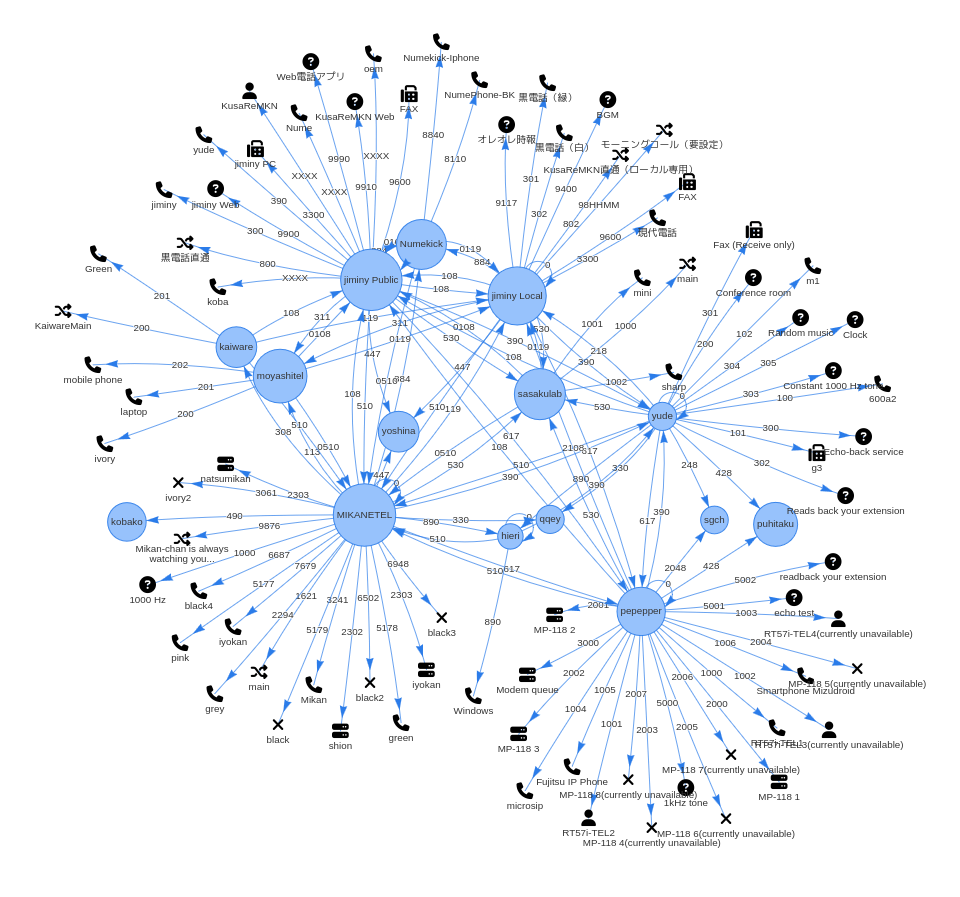
\includegraphics[height=.87\textheight]{./images/mantela.png}
    \end{column}
  \end{columns}
  \note{
    現在の電話網の姿を描画してみたよ。
    かなり小さくない網になっていることがわかると思うよ。

    この電話網の中には13個以上の電話局があって、
    端末数は58以上(隠されている端末もあるので実際には60数台)あるよ。
  }
\end{frame}

\begin{frame}
  \frametitle{現在の東京広域電話網の姿}

  \begin{columns}
    \begin{column}{.25\textwidth}
      \begin{description}[labelwidth=\linewidth]
        \item[交換局数]
          13局
        \item[端末数]
          58以上\\
          (仮想含む)
        \item[うち黒電話]
          10程度
        \item[その他]
          公衆電話\\
          ワープロ
      \end{description}
    \end{column}
    \begin{column}{.7\textwidth}
      \centering
      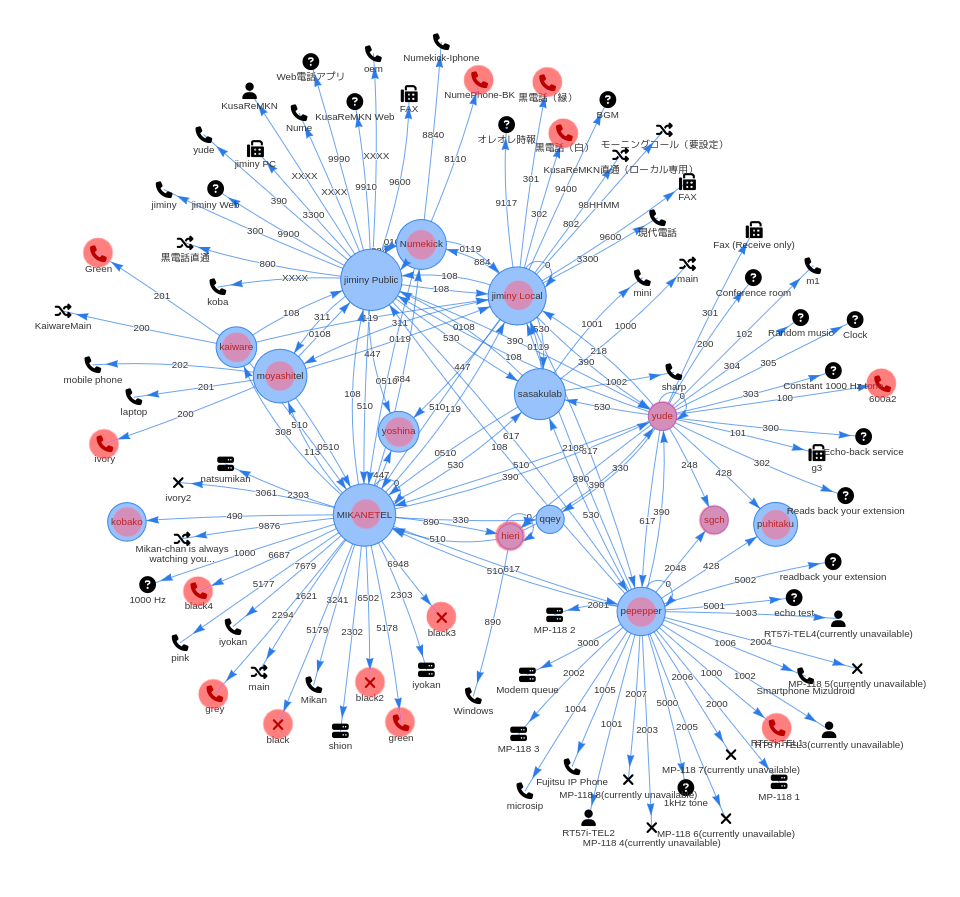
\includegraphics[height=.87\textheight]{./images/mantela2.png}
    \end{column}
  \end{columns}
  \note{
    もともと黒電話を使うことを念頭に作られた網であるので、
    黒電話を数えてみると10程度ありそうだよ。
    あ、この値は先週時点の値で、
    いまはちょっと増えているハズなので20弱くらいになっていそうだよ。

    その他にも、公衆電話が接続されていたり、
    ワープロが接続されていたりとかなり面白い網になっているよ。
  }
\end{frame}

\section{みんなも「でんわ」をしよう!}
\note{
  さて、ここまでの話を聞いて
  みんなも「でんわ」をしたくなっている頃だと思うので
  巻き込み活動を開始していくよ。
}

\begin{frame}
  \frametitle{用意するもの}

  必須なものは\textbf{コンピュータだけ}\\
  \hspace{1.5\zw}交換局を設置・相互接続するだけでOK
  \\~\\[-.5\baselineskip]

  黒電話やFAXなど物理的な端末をぶら下げたい場合は……

  \begin{description}[labelwidth=\linewidth]
    \item[VoIPルータ(ゲートウェイ?)]
      IP通信を電話信号に変換する人\\
      YAMAHA RT57iやRT58iなどで動作確認済\\
      ICOM VE-TA10もインチキすれば動作可能
    \item[端末それ自体]
      電話線の刺さるものはだいたい友達
  \end{description}
  \note{
    交換局を電話網に接続するだけであれば、
    必要なものは交換局だけなので、
    適当なコンピュータがあれば始められるよ(x86\_64であればOK)。

    実際の端末、例えば黒電話やFAXなどを接続するにはもう数品必要だよ。
    VoIPルータと端末それ自体だよ。
    VoIPルータはYAMAHAのものが安定して稼動しているよ。
    これはヤフオクやメルカリでよく手に入るという報告を受けているよ。
    黒電話も同様だよ。
    みんなもしようね。
  }
\end{frame}

\begin{frame}
  \frametitle{今日のお話の記事(宣伝(2回目))}

  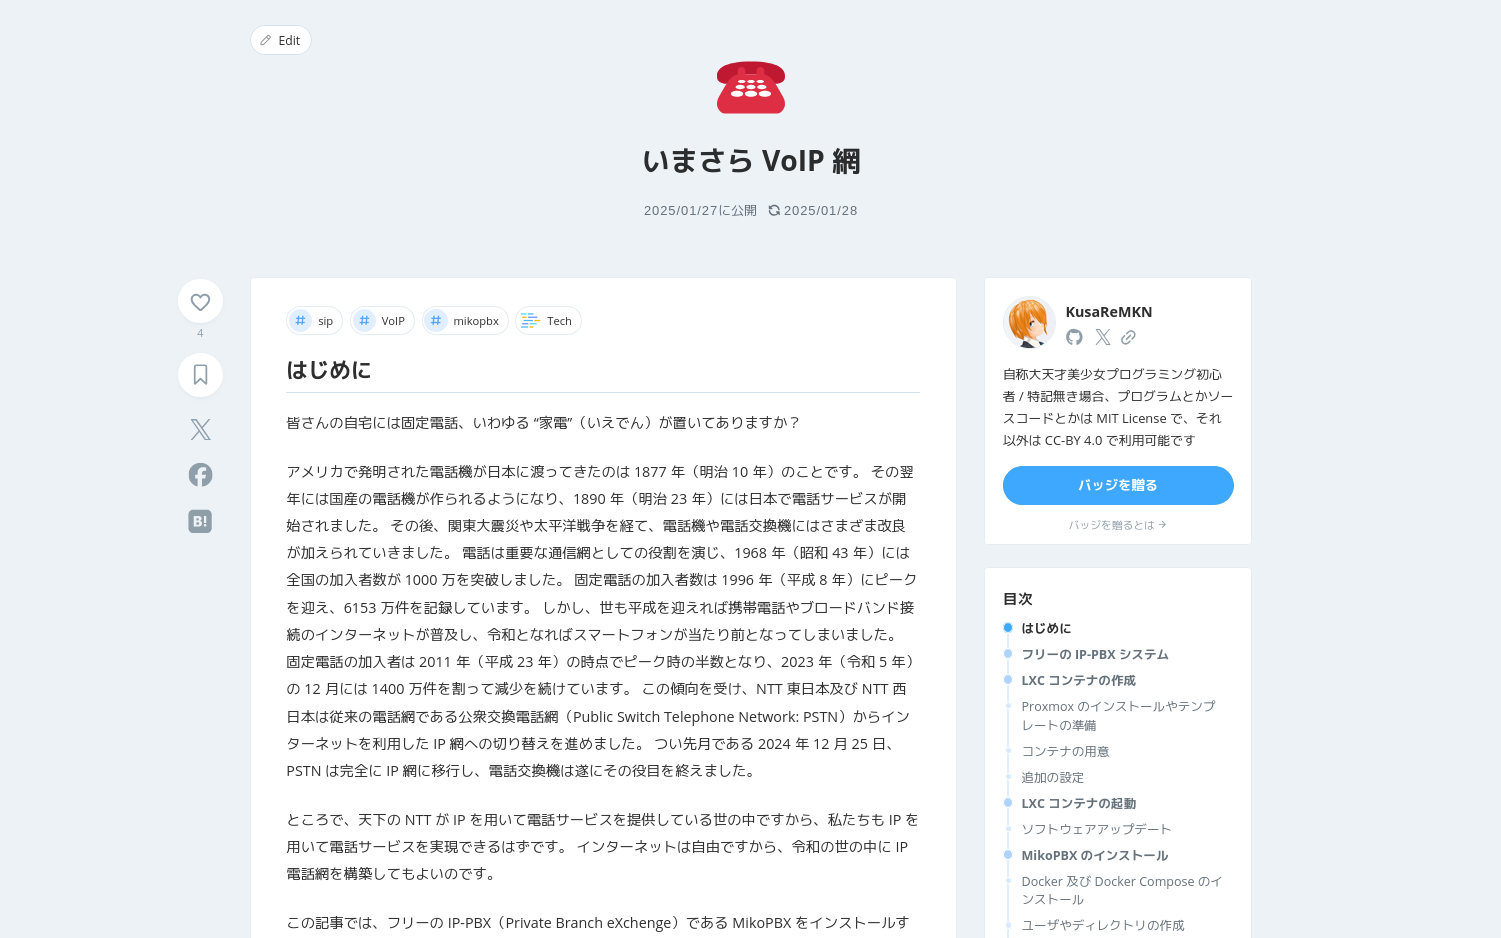
\includegraphics[width=\linewidth]{./images/imasara.png}
  \note{
    で、二回目の宣伝だよ。
    接続する方法の全てがZennに書いてあるよ。
  }
\end{frame}

\begin{frame}
  \frametitle{今日のお話の記事(宣伝(2回目))}

  \begin{description}[labelwidth=\linewidth,itemsep=\zh]
    \item[いまさらVoIP網]
      {\small
      \url{https://zenn.dev/kusaremkn/articles/abd760f9f2f450}}
    \item[VoIPルータを使って黒電話をIP電話機にする]
      {\small
      \url{https://zenn.dev/kusaremkn/articles/187222dc1d4f1d}}
    \item[ICOM VE-TA10を使うためにパケットを書き換えたりする]
      {\small
      \url{https://zenn.dev/kusaremkn/articles/cb32b500fc1334}}
  \end{description}
  \note{
    いまさらVoIP網でGoogleすると引っ掛かるハズなので、
    でんわをしてみたい人は検索してみてね。
  }
\end{frame}

\section{まとめ}
\note{
  今日のおはなしのまとめだよ。
}

\begin{frame}
  \frametitle{オレオレIP電話網と黒電話で遊んでみた}

  IP-PBXシステムを利用したIP電話網を構築

  交換局同士の相互接続・多局接続を実現

  交換局ホップの実現(相互接続されていない局間での通話)

  今後は電話網上のアプリケーションについて報告できたらいいな
  \note{
    オレオレIP電話網と黒電話で遊んでみたことについてお話をしたよ。
    MikoPBXというIP-PBXを用いてIP電話網を構築してみたよ。
    交換局同士の相互接続を実現できたし、
    多局接続を実現できたので本当に網になったよ。
    交換局ホップを実現して、
    直接相互接続されていない局でも通話できることを確認したよ。

    今後発表する機会があったら、
    電話網上のアプリケーションとかについて報告できたらいいな。
  }
\end{frame}

\begin{frame}[standout]
  おわりです
  \note{
    発表おわり〜
  }
\end{frame}

\begin{frame}
  \frametitle{このスライドについて}

  Written in February 2025.\\
  Updated in March 2025.\\
  \hspace{1.5\zw}Permanent ID of this document: \texttt{55b54dae70afe9e9}.
  \\~\\[-.5\baselineskip]

  Copyright © 2025 KusaReMKN.
  \\~\\[-.5\baselineskip]

  特記無き場合、プログラムやソースコードは MIT License で、\\
  \hspace{1.5\zw}それ以外のコンテンツは CC-BY 4.0 で利用可能です。\\
  \hspace{1.5\zw}一部の画像には別のライセンスが適用されるかもしれません。
\end{frame}

\end{document}
% ex: se et ts=2 :
